% AutoUI Work-in-Progress draft.
% Target venue: AutomotiveUI WIP track. Keep main text within the WIP page limit.
\documentclass[sigconf,review,anonymous]{acmart}
\settopmatter{printacmref=true}
\renewcommand\footnotetextcopyrightpermission[1]{}
\microtypesetup{expansion=false}
\hypersetup{%
  pdftitle={Auditable Driver-State Annotation from Naturalistic In-Cabin Video},
  pdfauthor={Anonymous Author(s)},
  pdfkeywords={Naturalistic driving, driver monitoring, glance annotation, human-in-the-loop, area of interest, hand-on-wheel}}
\acmConference[AutomotiveUI WIP]{AutomotiveUI Work-in-Progress Track}{2026}{}
\acmBooktitle{AutomotiveUI Work-in-Progress Track, 2026}
\acmYear{2026}
\copyrightyear{2026}
\setcopyright{none}
\acmDOI{}
\acmISBN{}

\begin{document}

\title{Auditable Driver-State Annotation from Naturalistic In-Cabin Video}

\author{Anonymous Author(s)}
\affiliation{%
  \institution{Anonymous Institution}
  \city{Anonymous}
  \country{Anonymous}}
\email{anonymous@example.com}

\begin{abstract}
Naturalistic driving studies increasingly rely on in-cabin video to study
driver attention and supervision, yet many datasets are collected without
synchronized eye tracking or frame-level driver-state labels. This gap
creates a methodological problem for downstream behavioral analysis:
researchers need scalable measures of where drivers look and whether
their hands remain on the steering wheel, but fully manual video coding
does not scale to long-duration, multi-participant recordings. This
work-in-progress paper presents an auditable human-in-the-loop workflow
for converting ordinary in-cabin video into area-of-interest (AOI) glance
categories and hand-on-wheel state variables. The workflow combines
reviewed driver-region specification, consensus AOI annotation,
participant-specific calibration, frame-level inference, temporal
stabilization, hand/wheel detection, hand/wheel state distillation,
and window-level behavioral metric extraction. We report preliminary
evidence from 15 naturalistic-driving
participants, including 301 processed gaze/wheel segments, approximately
3.91 million frame-level outputs, 7,306 coverage-qualified 20 s behavior
windows, a five-seed 14-participant leave-one-participant-out AOI
experiment, a no-leak few-shot adaptation curve, a temporal stabilization
ablation, hand-on-wheel review subsets, a GroundingDINO-to-YOLO
state-distillation check, and ONNX deployment checks. The
contribution is not a new gaze-estimation backbone or an eye-tracking
replacement. Instead, the paper defines a reusable annotation and
validation workflow for downstream studies that require transparent,
reviewable driver-state features from naturalistic video.
\end{abstract}

\begin{CCSXML}
<ccs2012>
   <concept>
      <concept_id>10003120.10003121.10011748</concept_id>
      <concept_desc>Human-centered computing~Empirical studies in HCI</concept_desc>
      <concept_significance>500</concept_significance>
   </concept>
   <concept>
      <concept_id>10010147.10010371.10010396</concept_id>
      <concept_desc>Computing methodologies~Computer vision tasks</concept_desc>
      <concept_significance>300</concept_significance>
   </concept>
</ccs2012>
\end{CCSXML}

\ccsdesc[500]{Human-centered computing~Empirical studies in HCI}
\ccsdesc[300]{Computing methodologies~Computer vision tasks}

\keywords{Naturalistic driving, driver monitoring, glance annotation, human-in-the-loop, area of interest, hand-on-wheel}

\maketitle

\section{Introduction}

Naturalistic driving studies are valuable because they preserve the
conditions under which driver supervision actually occurs: real traffic,
real vehicle interfaces, variable lighting, different cabin layouts, and
drivers who are not constrained by laboratory tasks. These strengths also
make the data difficult to analyze. Many in-cabin video datasets are
recorded with ordinary cameras rather than synchronized eye trackers. As
a result, they do not directly contain fixations, point-of-regard
estimates, or area-of-interest (AOI) glance labels. Before such datasets
can support questions about driver monitoring, distraction, takeover
readiness, or engagement with driver-assistance systems, researchers must
first turn video into behavioral variables.

Manual coding remains the most interpretable way to produce these
variables, but it is difficult to scale. Frame-level or clip-level coding
requires substantial labor, and reliability checks require preservation
of pre-consensus labels or review artifacts. These costs become a
bottleneck when a study grows from a small set of clips to hundreds of
segments and millions of frames. Fully automated computer vision is
appealing, but a black-box classifier is not sufficient for naturalistic
driving data. A visually plausible prediction can still be invalid if the
driver crop is wrong, if a passenger appears in the selected region, if a
face detector fails under glare or occlusion, or if a short prediction
flicker is interpreted as a behavioral event.

This paper treats driver-state extraction as a measurement workflow
rather than a single model score. Recent models provide useful building
blocks: YOLOv8-cls offers a compact train-export-deploy path for image
classification \cite{jocher2023ultralytics}; SCRFD provides face evidence
that can support driver-region review \cite{guo2021scrfd}; and
GroundingDINO can localize open-vocabulary objects such as hands and
steering wheels \cite{liu2023groundingdino}. However, these models do not
define the study geometry or the behavioral semantics by themselves. In
our workflow, humans specify or confirm driver regions, label AOI
semantics, review model outputs, and inspect uncertain hand-state cases.
Computer vision is used to extend those decisions across long video
segments while preserving checkpoints that can be audited.

The resulting measures should be interpreted as AOI-level driver-state
features, not continuous gaze estimates or substitutes for eye tracking
\cite{fridman2016drivergaze,saeJ2396,iso15007}. The workflow is intended
for downstream naturalistic-driving studies that need features such as
forward-roadway time, off-path glance episodes, in-vehicle glances, and
hands-on/off-wheel ratios. In this WIP, we make four contributions.
First, we describe a human-in-the-loop annotation workflow that separates
ROI provenance, AOI semantics, temporal stability, hand-state review, and
window-level aggregation. Second, we report preliminary evidence for the
main checkpoints using reviewable artifacts from 15 participants. Third,
we evaluate model and deployment choices so that the workflow can be
treated as a measurable annotation method rather than an undocumented
preprocessing step. Fourth, we add a state-distillation checkpoint for
the slow hand/wheel branch: GroundingDINO is used as a teacher on selected
frames, the resulting stable states are converted into a compact student
dataset, and the student is evaluated by teacher-state agreement and
runtime before any large-scale replacement is claimed.

\section{Workflow Design}

Figure~\ref{fig:workflow} summarizes the workflow. The input is a set of
target videos and analysis segments defined by a study spreadsheet. The
workflow resolves local videos, assigns or reviews driver regions,
constructs annotation packs, collects human AOI labels, trains
participant-specific AOI classifiers, exports deployment models, runs
segment-level inference, stabilizes frame-level predictions, estimates
hand-on-wheel states, optionally distills GroundingDINO teacher outputs
into a lightweight state student, and aggregates the
resulting streams into
behavioral windows.

\begin{figure}[t]
    \centering
    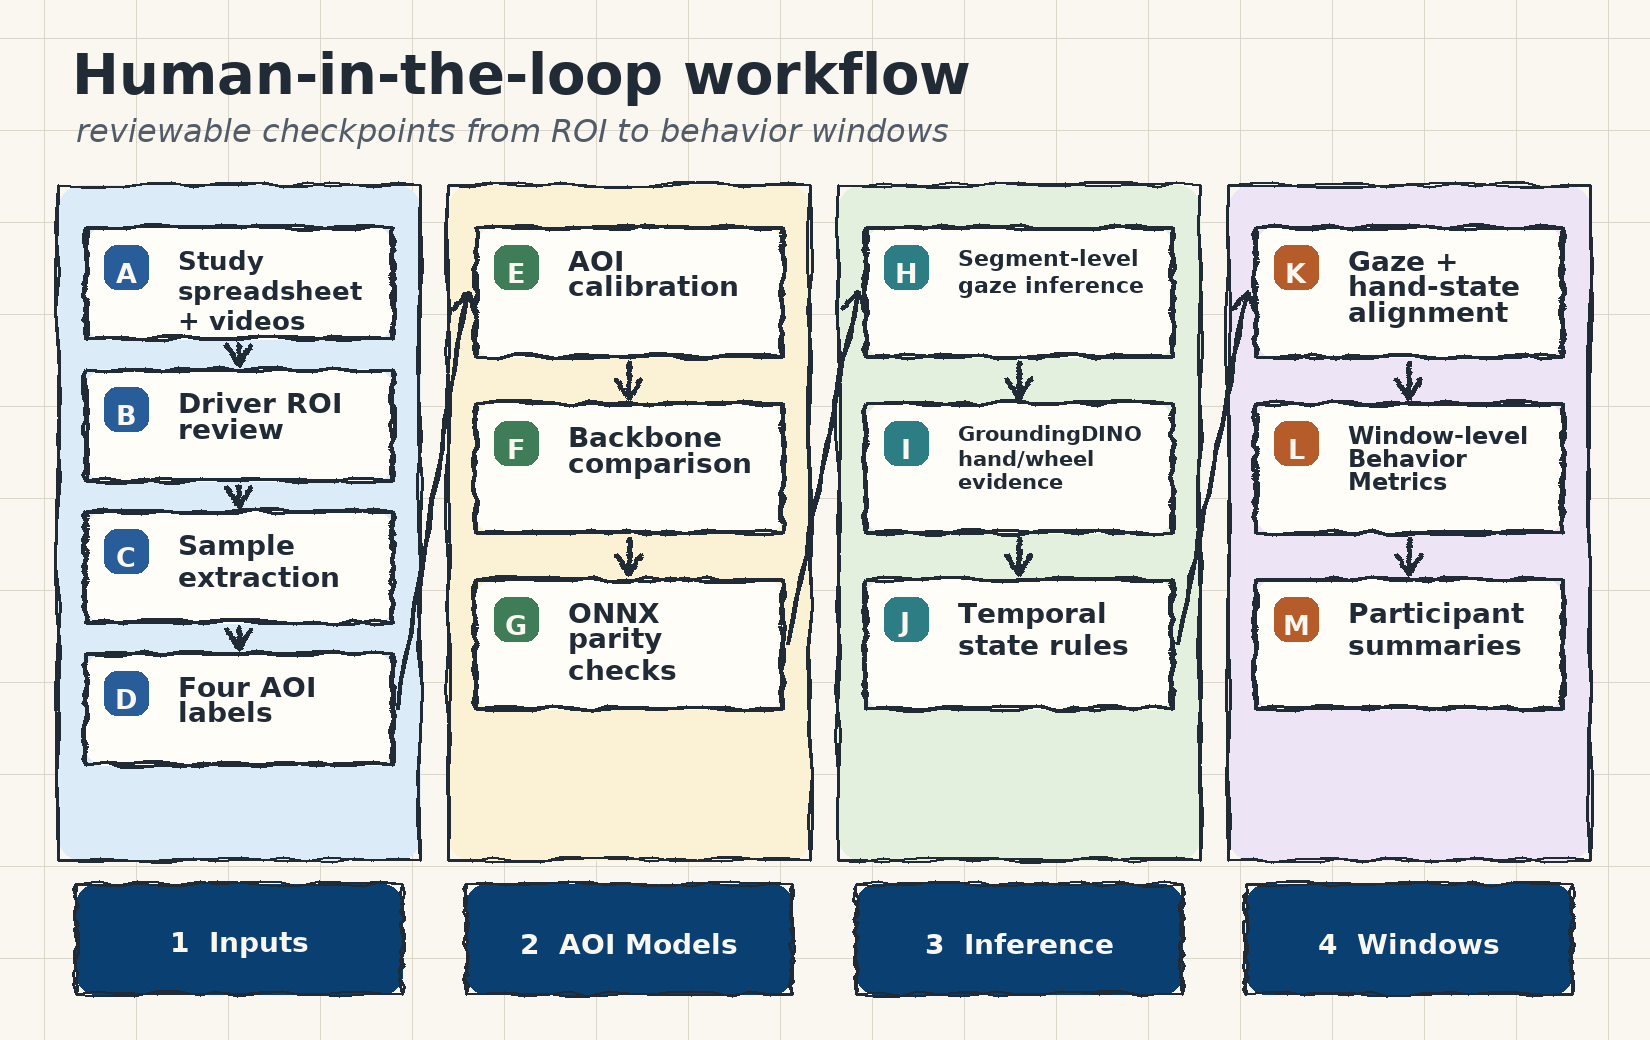
\includegraphics[width=\linewidth]{lable_workflow.png}
    \Description{A workflow diagram showing spreadsheet-defined target videos,
    human ROI specification, annotation packs, AOI model training, ONNX
    export, segment inference, temporal stabilization, and window-level
    behavior aggregation.}
    \caption{Human-in-the-loop workflow for deriving AOI-level glance and
    hand-on-wheel variables from naturalistic in-cabin video. The method keeps
    ROI provenance, frame semantics, temporal stability, hand-state review, and
    behavior aggregation as separate reviewable stages.}
    \label{fig:workflow}
\end{figure}

\subsection{Measurement Targets}

The gaze branch assigns each interpretable frame to one of three valid
AOI classes. \textit{Forward} denotes attention toward the forward
roadway. \textit{In-Car} denotes attention toward in-vehicle targets such
as the instrument cluster, center display, mirrors, or controls.
\textit{Non-Forward} denotes attention away from both the forward roadway
and in-vehicle targets. A fourth label, \textit{Other}, is used for
invalid or non-interpretable frames, including wrong ROI, no visible
driver, missing or unusable face evidence, non-target person, severe
artifact, or insufficient visual information. The primary behavior
metrics use the three valid AOI classes, while \textit{Other} is retained
for data cleaning, model training, and secondary error analysis.

The hand branch estimates steering-wheel engagement as \textit{ON},
\textit{OFF}, or \textit{UNCERTAIN}. These states are derived from hand
and steering-wheel detections, spatial contact evidence, and temporal
state rules. For window-level analysis, hand-state samples are aligned
with the gaze stream so that researchers can compute both overall and
AOI-conditioned hands-on/off ratios.

\subsection{Human ROI Specification}

ROI selection is treated as part of the measurement method rather than as
an invisible preprocessing step. In simple video layouts, a reviewer
records the driver ROI directly. In dual-panel or multi-view layouts,
face-detection evidence is used to rank candidate driver panels, but the
selected panel remains subject to visual confirmation. When automatic
assignment is uncertain, the workflow exports grid-overlay reference
images and fill-in manifests for manual correction. This design matters
because downstream AOI and hand-state predictions are only meaningful if
the crop contains the intended driver and the intended body region.

\subsection{Human AOI Annotation}

After ROI specification, representative frames are sampled across each
target video's temporal range and presented for human annotation. Coders
assign each ROI crop to \textit{Forward}, \textit{In-Car},
\textit{Non-Forward}, or \textit{Other}. The \textit{Other} class is not
treated as a nuisance afterthought. Naturalistic recordings often contain
systematic invalid samples caused by occlusion, lighting, camera layout,
or non-driver faces. Forcing these samples into a valid AOI would
contaminate both model training and downstream behavior summaries.

The annotation process is designed to preserve consensus decisions while
also documenting reliability limits. When coder-specific pre-consensus
labels are available, chance-corrected agreement can be reported with
Cohen's \(\kappa\) \cite{cohen1960coefficient}; Fleiss' \(\kappa\) is
appropriate only when more than two coders independently label the same
items \cite{fleiss1971}. In the current archive, consensus labels and
disagreement flags were retained, but complete coder-specific
pre-consensus vectors were not retained for every reviewed sample. We
therefore treat aggregate pre-consensus agreement as descriptive evidence
and report the absence of a reconstructable chance-corrected statistic as
a limitation.

\subsection{AOI Classification and Participant Adaptation}

The operational AOI branch uses a YOLOv8-cls classifier because it
provides a compact training and deployment path. Participant-specific
calibration starts from a small set of labeled samples and produces a
participant-adapted classifier for segment-level inference. At inference
time, SCRFD detects faces within the reviewed driver ROI; a
layout-specific target-face rule rejects implausible identity jumps and
selects the driver face; the selected crop is then classified into the
four AOI labels.

Because deployment convenience does not by itself establish measurement
validity, the repository also includes a model-comparison workflow that
trains YOLOv8-cls, ResNet, EfficientNet, ConvNeXt, and ViT backbones under
a common held-out-participant protocol. The comparison is not meant to
find a universally best backbone. It tests whether the deployment choice
has an irreplaceable accuracy advantage, and whether alternative
backbones remain viable when participant generalization or calibration
budget is the central concern.

\subsection{Temporal Stabilization}

Frame-level model outputs are not used directly as behavioral events.
Naturalistic video contains short face-detection dropouts, occlusions,
lighting transitions, and classifier flicker. The workflow applies
presence hysteresis and class debounce rules before computing
window-level metrics. Presence hysteresis prevents a brief missed
detection from immediately producing an invalid state. Class debounce
requires a candidate AOI label to persist before replacing the current
stable label. This separation keeps frame semantics and temporal event
structure analytically distinct: a classifier can be accurate at the
frame level while still producing behaviorally implausible flicker.

\subsection{Hand-on-Wheel State Estimation}

The hand branch uses the steering-wheel camera view. GroundingDINO
detects hands and steering wheels with open-vocabulary prompts. Contact
evidence is computed from overlap between detected hand boxes and
steering-wheel boxes. The frame-level state machine maps reliable contact
evidence to \textit{ON} or \textit{OFF}; unreliable frames retain the
previous state for a short grace period before entering
\textit{UNCERTAIN}. A temporal majority rule then produces the stable
state sequence used for review and metric extraction.

GroundingDINO is useful for bootstrapping because the target objects can
be specified by text prompts, but it is too slow to be the only detector
for repeated large-scale video processing. The workflow therefore treats
GroundingDINO as a teacher detector. Sampled teacher detections can be
exported to detection CSV files and reused in two distillation forms:
a two-class ROI-crop detector student with \textit{hand} and
\textit{steering wheel} labels, or a state-level ROI-crop classifier
student supervised by the teacher pipeline's stable
\textit{ON}/\textit{OFF}/\textit{UNCERTAIN} outputs. The latter is used
as the present acceleration checkpoint because the downstream analysis
consumes stable hand-state variables rather than raw boxes.

This branch is intentionally reviewed at the final-state level, after
detector confidence, contact rules, and temporal stabilization have acted
together. Reviewing only raw boxes would not show whether the derived
state sequence is behaviorally plausible. Reviewing only aggregate
hands-on percentages would hide whether failures come from the ROI,
detector, contact threshold, or temporal rule.

\subsection{Window-Level Metrics}

The stabilized gaze and hand-state streams are aggregated into fixed
analysis windows. Let \(g_i\) be the stabilized AOI label at time \(t_i\)
and let \(\mathcal{L}=\{\textit{Forward},\textit{In-Car},
\textit{Non-Forward}\}\) be the valid AOI set. Samples labeled
\textit{Other} are excluded from valid-AOI denominators. AOI time
percentages are computed with timestamp-based frame-duration weights
rather than raw frame counts, so the method can tolerate variation in
effective frame rate.

Glance counts are computed as entries into AOI episodes. Consecutive
frames with the same valid AOI label are treated as one episode. Long
off-path glances are defined as consecutive frames in either
\textit{In-Car} or \textit{Non-Forward}, with event counts reported at
1.6 s and 2.0 s thresholds. Hand-on-wheel ratios are computed overall and
conditioned on AOI label after excluding \textit{UNCERTAIN} and unmatched
wheel-state samples. Windows that fail the gaze-coverage threshold are
retained for quality control but excluded from participant-level behavior
summaries.

\section{Preliminary Evaluation}
\label{sec:preliminary_validation}

The evaluation focuses on whether the workflow produces reviewable
measurement artifacts, not whether it solves driver monitoring in a
single end-to-end score. Unless otherwise stated, the evidence below
reflects artifacts finalized by May 24, 2026, with processing coverage
finalized on May 25, 2026 for the 15-participant analysis set.

\begin{figure}[t]
    \centering
    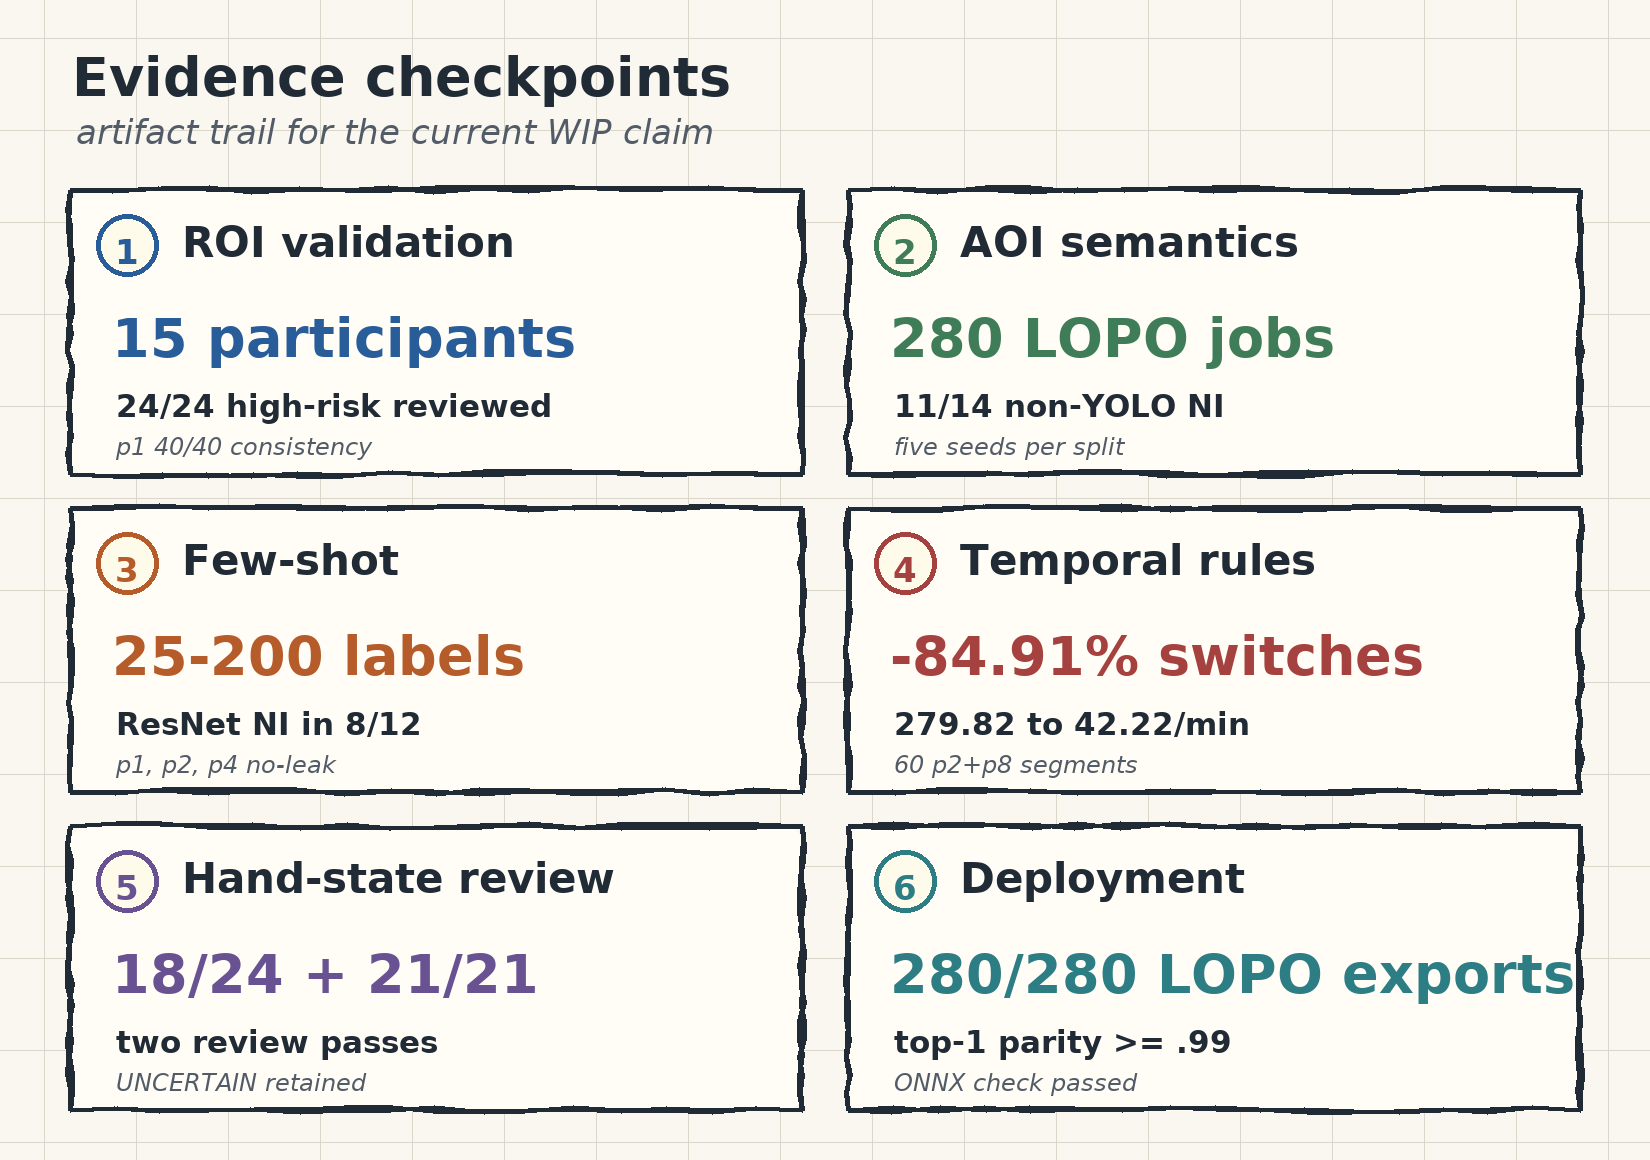
\includegraphics[width=\linewidth]{figures/evidence_checkpoints.png}
    \Description{A hand-drawn style diagram with six checkpoint boxes:
    ROI validation, AOI semantics, few-shot adaptation, temporal stability,
    hand-state review, and deployment. Each box contains a headline result
    from the evaluation artifacts.}
    \caption{Evidence checkpoints used to evaluate the annotation workflow.
    Each checkpoint corresponds to a distinct source of possible measurement
    error.}
    \label{fig:evidence_checkpoints}
\end{figure}

\subsection{ROI and Processing Coverage}

The ROI branch covers 15 participants with human-specified or
human-confirmed dual-ROI assignment files and production gaze/wheel ROI
manifests. The completed ROI audit covered provenance, resolution, and visual
validity of the production ROI set. Its high-risk portion included
uncertain p1 dual-ROI rows, p2 low-margin detector-assisted rows, and
later layout-specific gaze/wheel checks. All 24 high-risk rows were
reviewed to completion and resolved as confirmed, corrected, or
no-action cases. The p1 manual/current ROI consistency check matched
40/40 rows with zero coordinate changes.

The rebuilt inference plans, gaze maps, wheel maps, and 20 s behavior
windows cover all 15 analysis participants. Table~\ref{tab:coverage_refresh}
summarizes the resulting processing coverage. All 301 planned gaze/wheel
segments had frame-level CSV outputs, and all 7,327 generated windows
resolved to gaze and wheel files. The final participant-level summaries
used 7,306 windows that passed the 0.98 gaze-coverage threshold; 21
windows were retained for quality control but excluded from those
summaries.

\begin{table}[t]
\centering
\caption{Processing coverage across the 15-participant analysis set.}
\label{tab:coverage_refresh}
\resizebox{\linewidth}{!}{%
\begin{tabular}{lr}
\toprule
Coverage item & Value \\
\midrule
Participants in analysis & 15 \\
Matched target videos & 176 \\
Gaze segments with CSV outputs & 301 \\
Wheel segments with CSV outputs & 301 \\
Frame-level gaze rows & 3,914,416 \\
Frame-level wheel-state rows & 3,914,412 \\
Generated 20 s windows & 7,327 \\
Coverage-qualified windows & 7,306 \\
QC-excluded windows & 21 \\
\bottomrule
\end{tabular}
}
\end{table}

\subsection{AOI Generalization}

To evaluate cross-participant generalization, we ran a
leave-one-participant-out (LOPO) AOI experiment over 14 held-out
participants, five seeds, and four backbones, for 280 training runs. Each
split trains on all other participants and freezes the held-out
participant as the test set. The primary metric is three-class macro-F1
over \textit{Forward}, \textit{In-Car}, and \textit{Non-Forward};
\textit{Other} remains a secondary data-quality label because the
current test sets have limited invalid-sample support.

All 280 LOPO training runs and all 280 prediction jobs completed.
Table~\ref{tab:lopo_means} reports mean held-out performance across the
70 runs per model. ResNet50 achieved the highest mean three-class
macro-F1, balanced accuracy, and event-level accuracy. YOLOv8s-cls
remains a useful deployment baseline, but these multi-seed point
estimates do not show a unique accuracy advantage for YOLOv8s-cls.

\begin{table}[t]
\centering
\caption{Mean held-out performance in the five-seed 14-participant LOPO
AOI experiment. Each model has 70 held-out runs.}
\label{tab:lopo_means}
\begin{tabular}{lrrr}
\toprule
Model & Macro-F1 & Bal. acc. & Event acc. \\
\midrule
ResNet50 & 0.596 & 0.625 & 0.627 \\
EfficientNet-B0 & 0.575 & 0.601 & 0.616 \\
YOLOv8s-cls & 0.574 & 0.606 & 0.618 \\
DeiT-Tiny & 0.300 & 0.350 & 0.399 \\
\bottomrule
\end{tabular}
\end{table}

At the participant-split level, the best non-YOLO mean exceeded
YOLOv8s-cls on 11/14 participants. A bootstrap non-inferiority test with
a 3 percentage-point margin found at least one non-YOLO candidate
satisfying the margin on 11/14 splits. No non-YOLO model established
exact equivalence across the full \(\pm\)3 percentage-point band, so the
appropriate interpretation is family-best non-inferiority rather than
exact equality across all backbones or participants.

\subsection{Few-Shot Participant Adaptation}

The few-shot experiment tests how much participant-specific labeling is
needed when the goal is adaptation rather than zero-label
generalization. We ran a no-leak adaptation curve for p1, p2, and p4 at
25, 50, 100, and 200 label budgets, with five seeds per budget and
frozen participant-specific test sets. Figure~\ref{fig:fewshot_curve}
shows rapid ResNet50 gains from 25 to 100 labels, while YOLOv8s-cls
catches up and exceeds ResNet50 at 200 labels. The bootstrap
non-inferiority test found ResNet50 non-inferior to YOLOv8s-cls in 8/12
participant-budget cells. Thus, label budget and participant adaptation
are first-order design variables for this measurement workflow.

\begin{figure}[t]
    \centering
    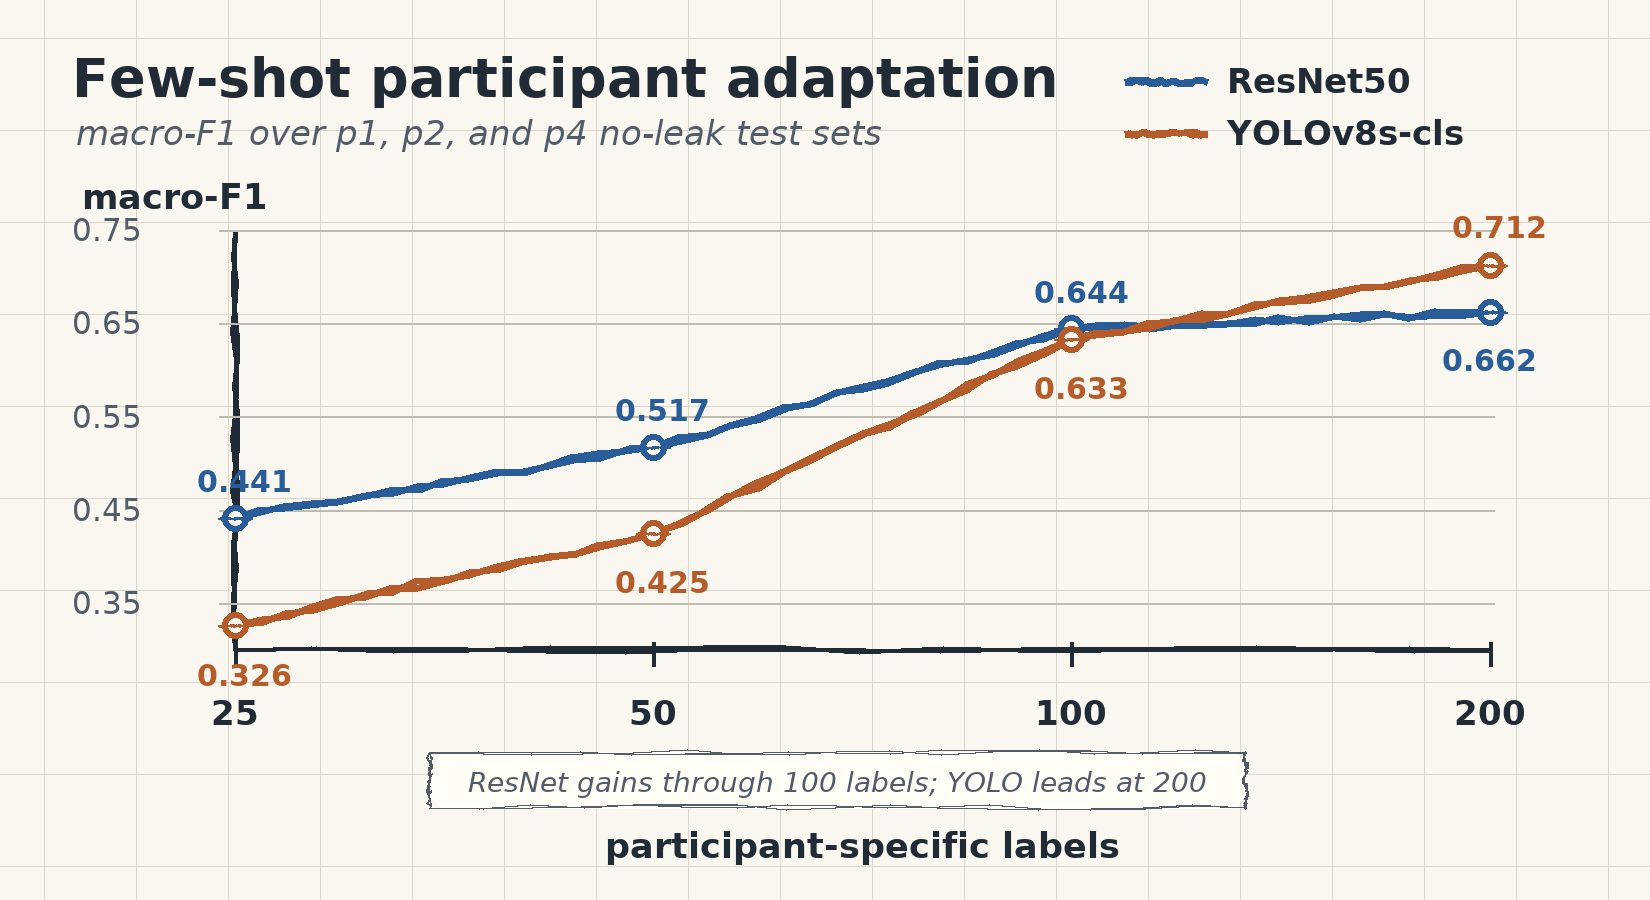
\includegraphics[width=\linewidth]{figures/fewshot_curve.png}
    \Description{A hand-drawn style line chart showing ResNet50 and
    YOLOv8s-cls macro-F1 over 25, 50, 100, and 200 participant-specific
    labels. ResNet50 rises quickly through 100 labels and YOLOv8s-cls is
    highest at 200 labels.}
    \caption{Few-shot no-leak adaptation curve over p1, p2, and p4
    (five seeds per participant-budget cell).}
    \label{fig:fewshot_curve}
\end{figure}

\subsection{Temporal Stability}

We compared raw per-frame AOI predictions with stabilized
\textit{Gaze\_Class} on a p2+p8 subset covering 60 segments, 643,603
frames, and 436.95 min. Stabilization reduced label switches from 279.82
to 42.22 per minute, an 84.91\% reduction. Raw and stable labels
differed on 106,418 frames, or 16.54\% of the subset. Stabilization also
changed behavior-level event structure: 1.6 s off-path episodes rose
from 923 to 1,289, and 2.0 s episodes rose from 696 to 1,032. These
results show why temporal rules must be evaluated directly rather than
treated as cosmetic smoothing.

\subsection{Hand-on-Wheel Review}

The wheel branch produced 301 segment-level outputs across all 15
analysis participants, totaling 3,914,412 state-classified rows. The
uncertainty rate remains high for several participants, including p15
with 75.2\% uncertain frames, p17 with 68.6\%, and p18 with 70.3\%.
These values indicate that hand-state estimation is more sensitive to
camera layout, occlusion, and steering-wheel evidence than AOI glance
classification.

The first agreement summary contained 24 reviewed rows with matched
pipeline and human labels. Agreement was 18/24 (75.0\%), with four
false-ON and two false-OFF cases. During review, we found that one
evidence batch initially reused single-panel gaze ROIs as wheel ROIs. We
therefore regenerated layout-specific cockpit evidence for the affected
participants. The corrected second pass covered seven participants and
21 final states; the reviewer judgment matched all 21 pipeline final
states, including 12 binary ON/OFF cases and nine \textit{UNCERTAIN}
cases (Table~\ref{tab:wheel_second_pass}). This supports plausibility
after ROI-evidence correction, while still leaving independent
double-coding as open work.

\begin{table}[t]
\centering
\caption{Hand-on-wheel final-state validation outcomes.}
\label{tab:wheel_second_pass}
\resizebox{\linewidth}{!}{%
\begin{tabular}{lrrr}
\toprule
Scope & Reviewed & Agreement & False ON/OFF \\
\midrule
Initial manifest & 24 & 18/24 & 4/2 \\
Corrected second pass & 21 & 21/21 & 0/0 \\
\bottomrule
\end{tabular}
}
\end{table}

\subsection{Hand/Wheel Distillation Check}

We ran a bounded state-distillation check to test whether slow
GroundingDINO hand/wheel inference can be amortized through a compact
student model. Two p1 GroundingDINO runtime probes, 60 s and 140 s, were
converted into 5,000 ROI crops labeled by the teacher pipeline's stable
\textit{ON}/\textit{OFF}/\textit{UNCERTAIN} state. A deterministic
frame-hash split held out 1,035 validation crops, including all three
states. A YOLOv8n-cls student trained from the local YOLOv8n-cls
checkpoint with low augmentation reached 0.988 top-1 teacher-state
accuracy by Ultralytics validation.

Table~\ref{tab:wheel_distill} summarizes the independent agreement and
runtime evidence. Re-running the saved student on the held-out validation
manifest produced 1,022/1,035 matching states, or 0.987 agreement with
the GroundingDINO teacher states. The confusion counts were
531 \textit{OFF}$\rightarrow$\textit{OFF},
12 \textit{ON}$\rightarrow$\textit{ON},
479 \textit{UNCERTAIN}$\rightarrow$\textit{UNCERTAIN},
and 13 total mismatches. After model loading and warm-up, the student
processed all 5,000 ROI crops in 6.342 s, or 1.268 ms per crop. The same
two GroundingDINO probes previously required 172.752 s, giving a
27.2$\times$ loaded-model speedup on the teacher-labeled probe set. This
check demonstrates distillation effectiveness without requiring the
remaining video segments to be re-inferred.

\begin{table}[t]
\centering
\caption{GroundingDINO-to-YOLO hand-state distillation check.}
\label{tab:wheel_distill}
\resizebox{\linewidth}{!}{%
\begin{tabular}{ll}
\toprule
Check & Result \\
\midrule
Teacher-labeled subset & 2 p1 probes; 5,000 ROI crops; 3 stable states \\
Split and student & 3,965 train / 1,035 validation; YOLOv8n-cls, 1.44M params \\
Teacher-state agreement & 0.987 validation agreement; 1,022/1,035 states match \\
Runtime probe & 6.342 s for 5,000 crops; 27.2$\times$ vs. GroundingDINO teacher wall time \\
\bottomrule
\end{tabular}
}
\end{table}

\subsection{Deployment Checks}

Deployment checks support the engineering feasibility of the workflow.
In the five-seed LOPO matrix, all 280 trained models exported to ONNX and
no top-1 parity result fell below 0.99. Table~\ref{tab:deployment}
reports a compact CPU benchmark from the holdout protocol, where all 120
exports completed. YOLOv8n/s are smaller and faster than the non-YOLO
backbones; ResNet50 is the fastest non-YOLO option but is much larger on
disk. These results support YOLOv8-cls as a convenient deployment path
even though it is not uniquely accurate in the held-out AOI experiments.

\begin{table}[t]
\centering
\caption{Compact ONNX CPU deployment benchmark from the holdout protocol.}
\label{tab:deployment}
\resizebox{\linewidth}{!}{%
\begin{tabular}{lrrrr}
\toprule
Model & MB & B1 p50 ms & B1 img/s & B32 img/s \\
\midrule
YOLOv8n-cls & 5.5 & 4.85 & 202.2 & 1621.2 \\
YOLOv8s-cls & 19.4 & 5.26 & 183.7 & 903.6 \\
ResNet50 & 89.6 & 7.20 & 139.1 & 525.7 \\
DeiT-Tiny & 21.2 & 17.19 & 56.7 & 291.1 \\
EfficientNet-B0 & 15.3 & 18.63 & 53.4 & 288.3 \\
ConvNeXt-Tiny & 106.2 & 18.65 & 51.8 & 114.1 \\
EfficientNet-B3 & 40.8 & 33.69 & 29.4 & 157.5 \\
\bottomrule
\end{tabular}
}
\end{table}

\section{Discussion}

The workflow addresses a recurring measurement problem in
naturalistic-driving research: studies often need driver-state variables
from long in-cabin videos, but the available data do not contain
eye-tracking streams or hand-state labels. The central design choice is
to keep the annotation process auditable. ROI selection, AOI semantics,
participant calibration, temporal stability, hand-state review, and
window aggregation are separate stages, so errors can be localized and
corrected rather than hidden inside an aggregate model score.

The preliminary evidence also clarifies the role of the computer-vision
backbones. YOLOv8-cls is attractive because it is compact, easy to train,
and straightforward to export. The AOI experiments, however, suggest
that deployment convenience should not be confused with unique accuracy.
ResNet50 and EfficientNet-B0 remain competitive under participant
generalization and few-shot adaptation. For hand-on-wheel estimation,
GroundingDINO is useful for open-vocabulary bootstrapping and review, but
its computational cost and uncertainty rates suggest that a smaller
task-specific student may be preferable for large-scale deployment. The
state-distillation check shows one practical route: spend the
GroundingDINO cost once on selected teacher frames, then use a compact
student classifier to reproduce stable hand-state outputs for faster
future inference.

For downstream studies, the practical value of this method is that it
turns video into documented behavioral variables without requiring each
study to re-derive the full annotation pipeline. A later analysis can cite
this workflow as the source of AOI glance and hand-on-wheel feature
construction, while focusing its own claims on the behavioral or
psychological question under study. That citation relationship requires
the present paper to remain method-focused: it defines the measurement
process, evidence checks, and limitations, but it does not claim the
substantive results of any downstream trust or automation-use analysis.

\section{Limitations and Open Work}
\label{sec:remaining_work}

Several limitations remain. First, the workflow depends on participant
labels and is not a zero-label generalization system. Second,
\textit{Other} is important for robustness but remains difficult to
evaluate when frozen test sets contain few invalid samples. Third, ROI
transcription or layout-selection errors can dominate downstream
results; the current production manifests have completed visual ROI
review, but new layouts, videos, or manifest edits would require repeated
review. Fourth, the corrected hand-on-wheel second pass is
single-reviewer evidence and should be expanded into an independently
double-coded validation set. Fifth, the current distillation check is
p1-derived and uses a frame-hash validation split, so the student should
be retrained and stress-tested on broader multi-participant teacher
samples before replacing GroundingDINO in production. Finally, deployment
benchmarks should be repeated on the target runtime hardware before
strong latency claims are made.

\section{Conclusion}

This WIP presents a human-in-the-loop workflow for extracting AOI-level
glance and hand-on-wheel variables from naturalistic in-cabin video. The
workflow combines human ROI review, AOI annotation, participant-specific
calibration, segment-level inference, temporal stabilization,
hand-on-wheel review, state distillation, and window-level metric
extraction. Preliminary evidence from 15 participants shows that the
pipeline can process millions of frames while preserving checkpoints for
ROI validity, AOI generalization, adaptation cost, temporal stability,
hand-state plausibility, student acceleration, and deployment
feasibility. The resulting contribution is a
transparent measurement method for downstream naturalistic-driving
studies, not a replacement for eye tracking or a standalone theory of
driver behavior.

\bibliographystyle{ACM-Reference-Format}
\bibliography{method_citation_entries}

\end{document}
